\chapter{Resultados}
\label{chap-results}

Esta Sección presenta un análisis de los resultados obtenidos de la ejecución del algoritmo sobre distintos videos. A lo largo de est Sección se refiere al algoritmo como a la modificación que se le hizo a \textit{contornos activos} y que fue descripta en el Capítulo \ref{chap-solution}. Las palabras \textit{aplicación} y \textit{programa} serán utilizadas indistintamente para referirse al programa que implementa dicho algoritmo, junto con una interfaz de usuario para el operador. Se refiere a la\textit{implementación} como a la parte del programa que implementa el algoritmo.

Se presentan los resultados obtenidos de la ejecución del programa, junto con métricas utilizadas para evaluar la performance de la implementación.

\section{Aplicación}

El programa incorpora una interfaz gráfica utilizada tanto para dar instrucciones como para recibir información acerca del partido y del funcionamiento del algoritmo. La misma cuenta con una sección donde se muestra una lista de jugadores siendo seguidos, otra donde se puede visualizar el video original con un recuadro en cada jugador seguido, un mapa de calor de espacios ocupados por los jugadores, y una imágen que permite al operador evaluar el correcto funcionamiento del algoritmo.

Para comenzar la ejecución, la implementación requiere que el operador identifique la posición de los jugadores en la imagen inicial de la secuencia. En este paso, también debe agregar información acerca del número de camiseta que viste, el equipo, y nombre del jugador.

Un paso adicional que debe ejecutar el operador es determinar puntos a utilizar para el cálculo de la homografía.

% TODO: Esto no se entiende, y no lo explicamos antes????
Los datos necesarios son al menos cuatro parejas de puntos. De estas parejas, el primer punto es una coordenada la imagen en perspectiva y el otro punto es la coordenada en un plano bidimensional. Con cuatro de estas relaciones, se puede calcular la matriz que resuelve la homografía para cualquier otro punto.  

Una vez que el programa tiene estos datos, el algoritmo de contornos activos puede comenzar a correr. Existen dos modos, uno que avanza sólo ante la indicación del operador (mecánica ``cuadro por cuadro'') y otro modo que avanza automáticamente cada vez que se computa un cuadro (mecánica ``tiempo real'').  % [ TODO: algo de amor a este párrafo ]

Para cada cuadro, una ventana muestra las posiciones actualizadas de los jugadores. El usuario puede seleccionar un jugador en particular y ver en detalle información sobre su posición, velocidad promedio, actual, y máxima desde el comienzo del seguimiento, y un mapa de calor que muestra con colores próximos al rojo los lugares más visitados por el jugador. Además, en un archivo se escribe la posición de cada jugador en cada momento.

De manera opcional, en cada cuadro se guarda en disco duro una copia del estado actual del seguimiento para referencia futura.

\section{Material utilizado}

Se utilizaron principalmente dos videos, uno correspondiente a un partido entre los equipos argentinos de los clubes Boca Juniors e Independiente; y un segundo video en el cual se enfrentan los equipos Independiente y San Lorenzo. Se detalla a continuación las características de las imágenes extraídas de esos videos.

\begin{itemize}
  \item \textbf{Boca vs Independiente:} El video cuenta con una resolución de \textit{1080p} (1920 pixels de ancho y 1080 de alto). La cancha se muestra en su totalidad, y se puede observar la totalidad de las gradas del lado opuesto y cielo por encima de ellas. Luego de descartar esas regiones del video, la resolución pasa a ser de 1459 píxels de ancho por 304 de alto. % TODO: No está terminado, falta describir jugadores y eso
  \item \textbf{Independiente vs San Lorenzo:} También filmado en resolución de \textit{1080p}, las esquinas del campo de juego quedan fuera del campo visual. Luego de descartar las gradas, la resolución final del video es de 1920 pixels de ancho y 540 de alto. % TODO: No está terminado, describir jugadores
\end{itemize}

Además, se tomaron pequeños cortes de tres videos de fútbol televisado en los cuales la cámara se encuentra relativamente estática y se analizó la correctitud del seguimiento en estos casos, contando con mayor resolución pero sin poder efectuar exitosamente la eliminación de fondo o la correlación a un plano bidimencional por homografía % [ TODO: ESTO ESTÁ ESCRITO CON LA ** ]

\begin{itemize}
  \item \textbf{Manchester City vs Barcelona:}
  \item \textbf{Real Madrid vs Borussia Dortmound:}
  \item \textbf{Argentina vs Suiza:}
\end{itemize}

\section{Evaluación del método}

Se evaluó cualitativamente por un operador que los contornos de los jugadores según el algoritmo modificado de contornos activos no correspondían a los jugadores, como es el caso de trabajos citados en el estado del arte (ver \cite{papers-tanos}). Se atribuye esto a la baja calidad de los videos que se pudieron obtener, y la poca capacidad de procesamiento en comparación. (TODO: Completar esto justificando mejor).

Dado esto, se procedió a evaluar cuántas veces sucedía esta discrepancia por unidad de tiempo. Esta métrica, resumida como la cantidad de errores del algoritmo por cada cien cuadros, se intentó minimizar durante el estudio de las variantes de la aplicación.

Otra métrica que se buscó minimizar es el tiempo de demora por cuadro procesado, hasta intentar alcanzar una velocidad de $24$ cuadros por segundo (equivalente a $42$ milisegundos por cuadro), la velocidad de los videos utilizados.

% TODO chequear la forma de referirse a NUESTRO algoritmo sin decir la palabra NUESTRO :s
%% TODO: Ojo, a partir de acá hablamos en pasado. Deberíamos ser consistentes,
%% por como arrancamos en el resuemen, la intro y por lo que dice la mina
%% deberiamos usar el presente o eso de "se plantea, se define, etc..."

\section{Comparación con IFTrace}
\label{sec:iftrace}

El algoritmo de seguimiento IFTrace, propuesto por \citeauthor*{IFTrace}, es un
algoritmo robusto que soporta cambios de iluminación y forma, oclusiones y se
centra en hallar características representativas de la textura de los objetos a
seguir. Es capaz de recuperarse de errores menores y permite el seguimiento de
múltiples objetos a la vez.

Un algoritmo de este tipo podría proporcionar una solución al problema. Para
comprobarlo, se llevaron a cabo algunas pruebas utilizando un video sintético
creado para este fin, y un video real de un partido de fútbol. En las Figuras
\ref{fig:sample-happy-occluded} y \ref{fig:sample-boca} pueden observarse los
primeros cuadros de cada video. Pueden apreciarse a simple vista las marcadas
diferencias entre ambos videos, como por ejemplo la resolución de la imagen y
el tamaño y la complejidad de los objetos de inteŕes.

\begin{figure}[H]
    \centering
    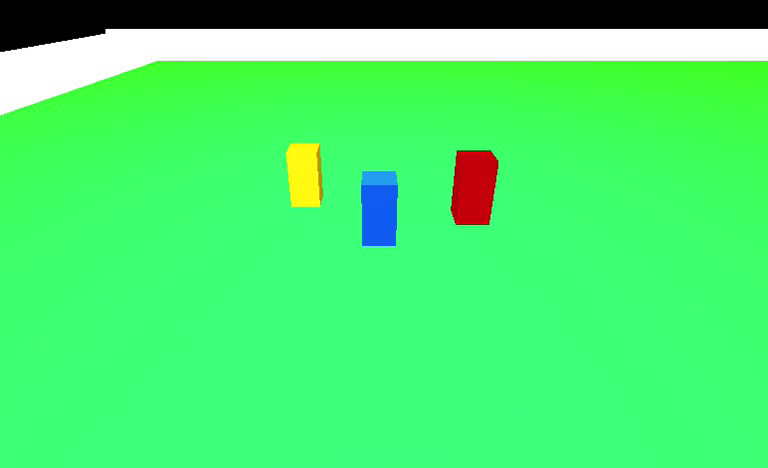
\includegraphics[width=\linewidth]{./images/sample_happy_occluded.png}
    \caption{Muestra de un cuadro del video sintético de prueba.}
    \label{fig:sample-happy-occluded}
\end{figure}

\begin{figure}[H]
    \centering
    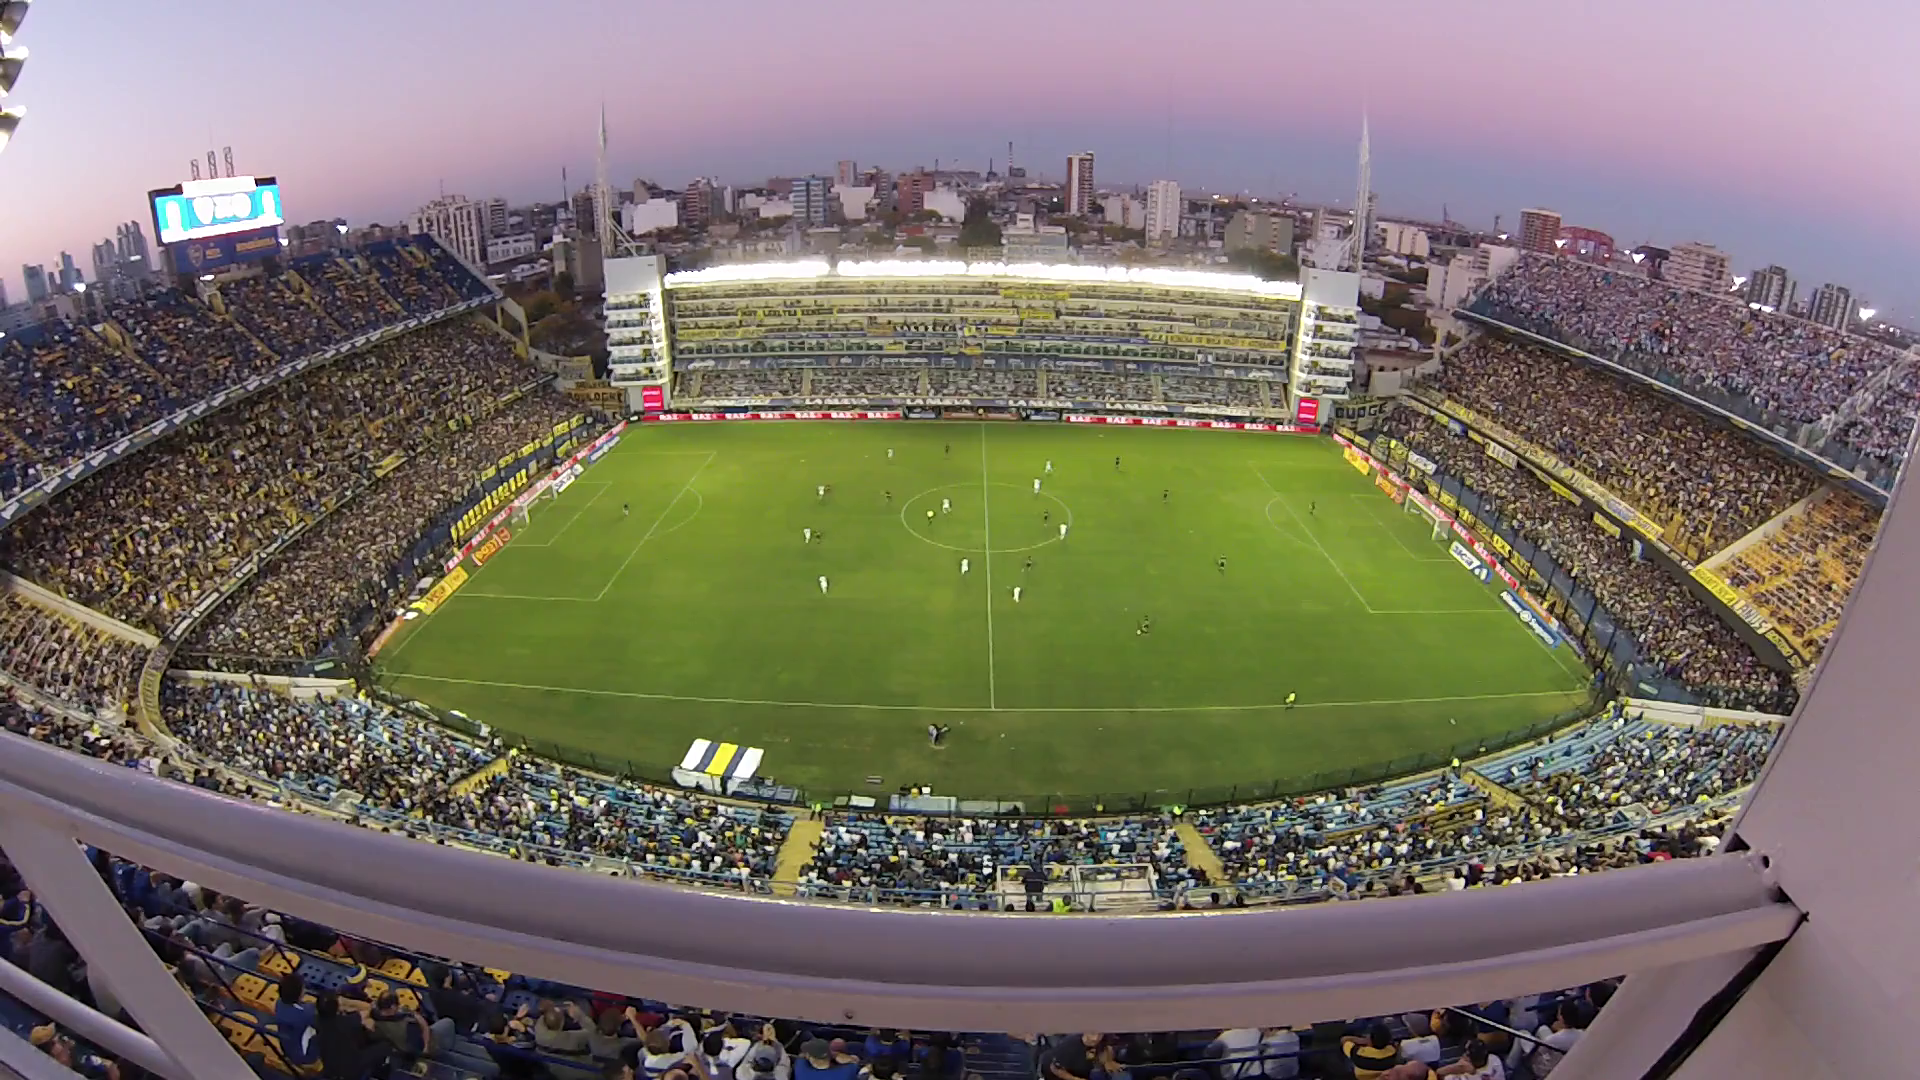
\includegraphics[width=\linewidth]{./images/sample_boca.png}
    \caption{Muestra de un cuadro del video real de un partido de fútbol.}
    \label{fig:sample-boca}
\end{figure}

Como se puede ver en la Figura \ref{fig:happy-occluded-iftrace}, IFTrace logra
un correcto seguimiento de múltiples objetos en el video sintético.  También
puede observarse, en la Figura \ref{fig:boca-iftrace}, como sigue correctamente
a un jugador en el video real.  Sin embargo, el seguimiento sólo es exitoso
durante unos pocos cuadros, ya que, en el cuadro 17, el algoritmo cae en un
error del cual sólo una corrección manual puede sacarlo. Este tipo de correción
semi-supervisada no está contemplada en el algoritmo de IFTrace.

\begin{figure}[H]
    \centering
    \begin{tabular}{cccc}
        \subfloat[Cuadro 1]{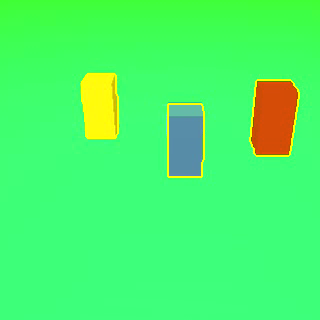
\includegraphics[width = 1.5in]{./images/cropped_happy_occluded_00001.png}} &
        \subfloat[Cuadro 5]{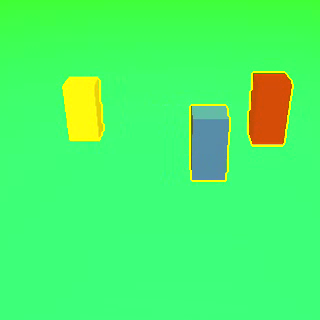
\includegraphics[width = 1.5in]{./images/cropped_happy_occluded_00005.png}} &
        \subfloat[Cuadro 8]{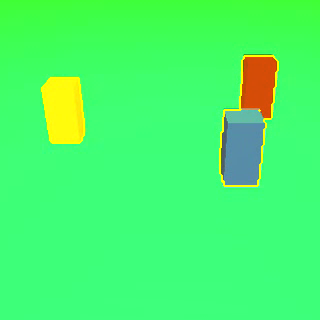
\includegraphics[width = 1.5in]{./images/cropped_happy_occluded_00008.png}} &
        \subfloat[Cuadro 12]{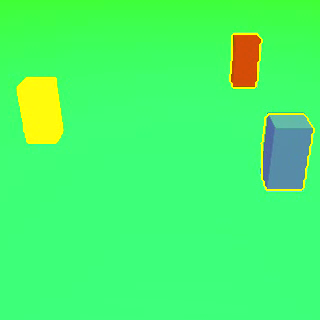
\includegraphics[width = 1.5in]{./images/cropped_happy_occluded_00012.png}}
    \end{tabular}
    %% NASTY hack to make refernce work with figures and subfigures, put \label inside \caption env, little bird told me
    \caption{IFTrace funcionando en una secuencia de cuadros de video sintético.
    \label{fig:happy-occluded-iftrace}
    }
\end{figure}

\begin{figure}[H]
    \centering
    \begin{tabular}{cccc}
        \subfloat[Cuadro 9]{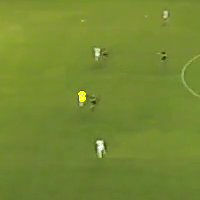
\includegraphics[width = 1.5in]{./images/cropped_boca_00009.png}} &
        \subfloat[Cuadro 12]{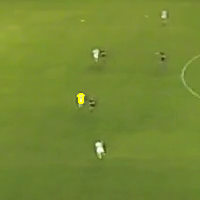
\includegraphics[width = 1.5in]{./images/cropped_boca_00012.png}} &
        \subfloat[Cuadro 14]{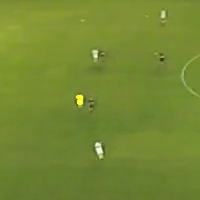
\includegraphics[width = 1.5in]{./images/cropped_boca_00014.png}} &
        \subfloat[Cuadro 17]{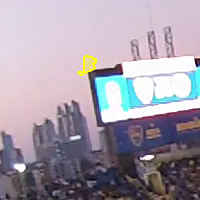
\includegraphics[width = 1.5in]{./images/cropped_boca_00017.png}}
    \end{tabular}
    %% NASTY hack to make refernce work with figures and subfigures, put \label inside \caption env, little bird told me
    \caption{Seguimiento de un jugador en un video real utilizando IFTrace.
    \label{fig:boca-iftrace}
    }
\end{figure}

\begin{figure}[H]
    \centering
    \begin{tabular}{cccc}
        \subfloat[Cuadro 1]{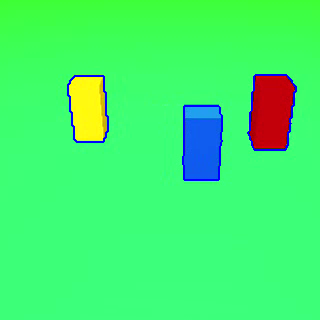
\includegraphics[width = 1.5in]{./images/cropped_processing2.png}} &
        \subfloat[Cuadro 5]{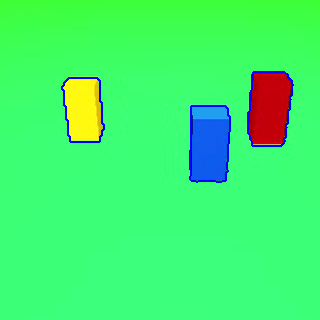
\includegraphics[width = 1.5in]{./images/cropped_processing5.png}} &
        \subfloat[Cuadro 8]{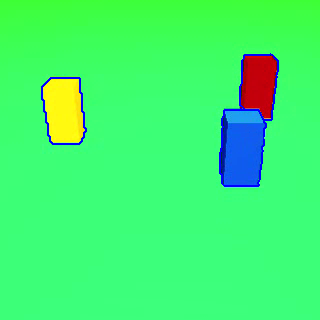
\includegraphics[width = 1.5in]{./images/cropped_processing14.png}} &
        \subfloat[Cuadro 12]{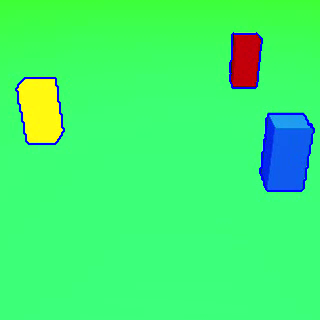
\includegraphics[width = 1.5in]{./images/cropped_processing25.png}}
    \end{tabular}
    %% NASTY hack to make refernce work with figures and subfigures, put \label inside \caption env, little bird told me
    \caption{Nuestro algoritmo en funcionamiento en un video sintético.
    \label{fig:happy-occluded-activeContour}
    }
\end{figure}

\begin{figure}[H]
    \centering
    \begin{tabular}{cccc}
        \subfloat[Cuadro 2]{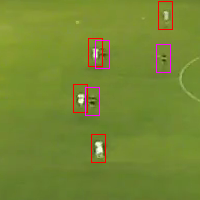
\includegraphics[width = 1.5in]{./images/cropped_rendered002.png}} &
        \subfloat[Cuadro 12]{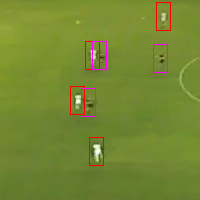
\includegraphics[width = 1.5in]{./images/cropped_rendered007.png}} &
        \subfloat[Cuadro 14]{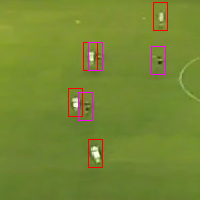
\includegraphics[width = 1.5in]{./images/cropped_rendered012.png}} &
        \subfloat[Cuadro 17]{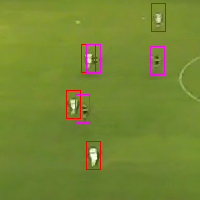
\includegraphics[width = 1.5in]{./images/cropped_rendered017.png}}
    \end{tabular}
    %% NASTY hack to make refernce work with figures and subfigures, put \label inside \caption env, little bird told me
    \caption{Seguimiento de los jugadores en un video real mediante el algoritmo de contornos activos modificados.
    \label{fig:boca-activeContour}
    }
\end{figure}

Como se puede observar en la Figura \ref{fig:happy-occluded-activeContour},
el algoritmo de contornos activos modificado logra seguir con éxito a los
objetos de interés en el video sintético. Además, también se obtiene un
resultado positivo en el video real en la situación en que IFTrace pierde al
jugador, como puede observarse en la Figura \ref{fig:boca-activeContour}.

\subsection{Evaluación de comportamiento}

Otro punto importante de comparación entre los dos algoritmos es su tiempo de
ejecución, es decir el tiempo que tarda en llevar a cabo su trabajo.  De
acuerdo a las mediciones realizadas con un video real de un partido de fútbol,
siguiendo a un solo jugador, el tiempo promedio que tarda IFTrace por cuadro es
6.962 segundos, mientras que nuestro algoritmo tiene un tiempo promedio de
0.712 segundos. Se puede observar que se encuentra un orden magnitud por debajo
de IFTrace.
%% 6.9628571428571435 si quieren los decimales
%% TODO verificar nuestro numero!!!

Cabe destacar que ambos algoritmos podrían verse beneficiados de ciertas
optimizaciones, como ser por ejemplo la programación en GPU y la reducción de
operaciones de \textit{Input/Output} al almacenamiento secundario (disco duro).

% TODO Esto creo que probablemente terminemos sacandolo right? Que métrica podemos meter?!?!
% - Comparación de nuestros resultados vs los de ellos (Métrica: cantidad de jugadores perdidos por frame -- o si se nos ocurre una mejor ambas o esa)

